\documentclass[preprint,12pt]{elsarticle}

\usepackage{amsmath,amssymb}
\usepackage{booktabs,tabularx,threeparttable,array,multirow}
\usepackage{graphicx}
\usepackage[ruled,vlined,linesnumbered]{algorithm2e}
\usepackage{tikz}
\usetikzlibrary{arrows.meta,positioning,fit,shapes.geometric}
\usepackage{xcolor}
\usepackage{microtype}
\usepackage{url}
\usepackage[hidelinks]{hyperref}
\usepackage{siunitx}
\usepackage{enumitem}
\usepackage{float}
\usepackage{pdflscape}
\usepackage{caption}
\usepackage{subcaption}
\captionsetup{font=small,labelfont=bf}

\journal{Building and Environment}

\begin{document}
\begin{frontmatter}

\title{Beyond Accuracy: Identifiability and Reliability Limits of Cross-System HVAC Fault Diagnosis under Distribution Shift}

\author[scu]{Chun-Jan Tseng\corref{cor1}}
\ead{cjtseng@scu.edu.tw}
\author[ndu]{Yi-Kai Su}
\author[nycu]{Ming-Han Chang}

\cortext[cor1]{Corresponding author.}
\address[scu]{Department of Data Science, Soochow University, Taipei 111002, Taiwan, ROC}
\address[ndu]{Department of Financial Management, National Defense University, Taipei 112305, Taiwan, ROC}
\address[nycu]{Department of Industrial Engineering and Management, National Yang Ming Chiao Tung University, Hsinchu 300093, Taiwan, ROC}

\begin{abstract}
Cross-system deployment of heating, ventilation, and air-conditioning (HVAC) fault detection and diagnosis (FDD) models is often judged from target classification scores, yet a low target score can arise for two different reasons: the fault distinction may never have been reliably identifiable at source, or a distinction learned at source may fail after transfer. Confidence metrics can be equally misleading when low selective risk is achieved by rejecting the fault classes that matter for maintenance. We formalize these distinctions through the Observability--Identifiability--Reliability framework for HVAC FDD (OIR-FDD), together with two deterministic audit algorithms. Identifiability-Gated Transfer Interpretation (IGTI) permits a transfer-failure claim only after source identifiability is established, while Class-Retention Reliability Audit (CRRA) evaluates calibration and abstention jointly with fault-class retention and persistent sensor-loss stress. The primary experiment transfers binary normal-versus-abnormal diagnosis from simulated to laboratory rooftop-unit (RTU) data with differing fault mechanisms. A supporting series-to-parallel fan-powered-unit transfer provides class-specific evidence. Eight baseline model families, source-only calibration, selective prediction, persistent dropout, fallback models, and semantic/graph ablations are evaluated under frozen source-governed rules. Target expected calibration error increases for all eight RTU baseline pipelines. A source-normal out-of-distribution (OOD) score rejects both target-normal and target-fault operation, showing domain-wide separation rather than fault-specific novelty. In the supporting cross-system experiment, valve-stuck recall falls from about 0.89 at source to 0.004--0.088 on target after source-side validation, whereas the two fouling mechanisms remain weak or unresolved at source. A selective-prediction counterexample attains zero aggregate risk while accepting none of the retained fault classes. Persistent sensor loss produces metric-dependent failures, and structural ablations show that clean-score gains from graph variants do not translate into consistent class-aware reliability. These results support a layered interpretation of HVAC transfer experiments in which physical eligibility, source discrimination, transfer performance, confidence, and sensing robustness are treated as separate evidence claims.
\end{abstract}

\begin{keyword}
HVAC fault diagnosis \sep cross-system transfer \sep source identifiability \sep calibration \sep selective prediction \sep sensor missingness \sep reliability benchmark
\end{keyword}

\end{frontmatter}

\section{Introduction}
Heating, ventilation, and air-conditioning (HVAC) fault detection and diagnosis (FDD) has progressed from expert rules and analytical residuals to supervised, semi-supervised, self-supervised, transfer-learning, graph-based, and agentic approaches \cite{katipamula2005a,katipamula2005b,kim2018review,mirnaghi2020review,chen2022review,chen2023review,bi2024review}. The practical motivation is well established: building-system faults can waste energy, degrade indoor conditions, and increase maintenance burden, while building automation systems provide large streams of sensor and control data that can support automated diagnosis \cite{shi2019review,andersen2024barriers}. Public fault datasets spanning simulation, laboratory facilities, and field operation now make reproducible model development possible \cite{granderson2023dataset}. At the same time, recent work has moved beyond within-dataset accuracy toward cross-building transfer, unsupervised domain adaptation, open-set diagnosis, ontology-supported reasoning, and real operational testing \cite{lei2025,zhang2025source,ghalamsiah2025can,ghalamsiah2026graph,gao2026open,li2026agentic,wang2026cross,mosteiro2026dbn}.

That progress creates a harder evaluation problem. A fault label attached to a file does not imply that every time window contains a physically informative fault signature. Even when the fault can manifest under the current operating condition, the available measurements may not distinguish one mechanism from another. Consequently, a low target score does not automatically diagnose ``transfer failure'': it can also reflect a source task that was only weakly learnable. The same distinction matters for confidence. A model can be well calibrated at source and miscalibrated after shift, or it can attain low error among accepted predictions by rejecting all maintenance-relevant faults. Sensor loss adds another layer because building FDD depends on the measurement roles that remain available \cite{zhang2021sensor,hu2025sensorreview,li2025voting}.

The literature already contains several pieces of this problem. Cross-building HVAC studies develop single- and multi-source adaptation strategies \cite{lei2025}, source-domain selection rules \cite{zhang2025source}, contrastive adaptation \cite{ghalamsiah2025can}, graph-based adaptation \cite{ghalamsiah2026graph}, and attention-based transfer \cite{wang2026cross}. Open-set work addresses unknown faults \cite{gao2026open}, and a recent leakage-safe air-handling-unit (AHU) study explicitly examines adaptation reliability, negative transfer, and confidence triage under limited target information \cite{jiang2026leakage}. General machine-learning research likewise shows that calibration and uncertainty can degrade under dataset shift \cite{guo2017calibration,ovadia2019uncertainty}, while selective prediction studies formalize the risk-coverage trade-off \cite{geifman2017selective,geifman2019selectivenet}. These contributions mean that neither domain shift nor reliability-aware evaluation is new by itself.

Our question is narrower and operational. Before a target failure is interpreted as transfer degradation, was the diagnostic distinction physically eligible and demonstrably identifiable at source? After transfer, does an apparent confidence improvement remain credible when fault-class retention and persistent sensor-loss stress are examined? We formalize this logic through the Observability-Identifiability-Reliability framework for HVAC FDD (OIR-FDD). OIR-FDD is an evaluation and claim-governance architecture rather than a new classifier. It contains two deterministic audit algorithms: Identifiability-Gated Transfer Interpretation (IGTI), which assigns class-specific transfer interpretations only after source identifiability is checked, and Class-Retention Reliability Audit (CRRA), which prevents aggregate calibration or selective-risk gains from being interpreted independently of retained fault recognition and worst-condition sensing stress.

Two complementary experiments are used. The primary experiment transfers binary normal-versus-abnormal diagnosis from simulated RTU data to laboratory RTU operation. The source and target contain different fault mechanisms, so this is a generation-domain reliability test rather than closed-set same-fault transfer. The supporting experiment transfers four-class diagnosis from a series fan-powered unit (SFPU) to a parallel fan-powered unit (PFPU). There, valve stuck is strongly identifiable at source and then collapses on target, while air-side and water-side fouling remain weak or unresolved at source. The combination makes it possible to distinguish credible transfer degradation from source-identifiability limits.

The study makes four contributions. First, it formalizes OIR-FDD as a layered framework linking physical eligibility, source identifiability, transfer interpretation, and class-aware reliability. Second, IGTI operationalizes the source-identifiability gate, while CRRA couples calibration and abstention with fault-class retention and persistent-dropout stress. Third, the framework is evaluated with eight baseline model families and frozen source-only decisions across two different HVAC transfer settings. Fourth, a dedicated structural-ablation study tests raw, functional, semantic, physical-graph, Brick-supported, hybrid, identity, and shuffled variants, preserving negative evidence when clean-score gains do not survive reliability stress. The framework does not claim field efficacy, universal HVAC behavior, or a new predictive architecture.

\section{Related work}
\subsection{HVAC FDD foundations, datasets, and evaluation practice}
Classical reviews organized building FDD around analytical, knowledge-based, and process-history approaches and highlighted the importance of detectability, isolability, sensor quality, and practical implementation \cite{katipamula2005a,katipamula2005b,kim2018review,yu2014ahureview}. Subsequent surveys document the rapid expansion of data-driven HVAC diagnosis, including supervised, unsupervised, hybrid, and deep-learning approaches \cite{mirnaghi2020review,chen2022review,chen2023review,bi2024review,singh2022review}. The operational literature also shows that deployment barriers are not purely algorithmic: data quality, commissioning practice, explainability, engineering effort, sensor availability, and organizational workflow remain important \cite{shi2019review,andersen2024barriers}.

Representative methods span rule-based AHU diagnosis \cite{schein2006rule}, chiller classification with discriminant analysis \cite{li2016lda}, semi-supervised chiller diagnosis \cite{beghi2016chiller}, associative classification \cite{huang2018assoc}, Bayesian networks with rejection and non-sensor information \cite{wang2017bayes}, and real-building frameworks based on operational building automation system (BAS) data \cite{soultanzadeh2024framework}. More recent work explores self-supervised time-series representation learning \cite{wang2026selfsup} and whole-building diagnostic Bayesian networks with operational testing \cite{mosteiro2026dbn}. These studies illustrate why a single accuracy score cannot describe the diversity of diagnostic tasks, sensor contracts, and deployment conditions.

Adjacent work by the authors on building-load multi-task learning and physics-informed industrial benchmarking also motivates explicit separation of model construction from evaluation contracts and deployment claims \cite{liu2023load,su2026pdm}; those studies are cited for methodological context rather than as HVAC-FDD evidence. The Lawrence Berkeley National Laboratory (LBNL) labeled HVAC collection is particularly relevant because it spans common commercial HVAC configurations and includes simulation, laboratory, and field data under multiple fault types and severities \cite{granderson2023dataset}. The availability of such data enables cross-system experiments, but it also increases the need to distinguish file-level fault presence from window-level physical support, split integrity, source learnability, and field generalization.

\subsection{Cross-domain, simulation-to-real, and open-set diagnosis}
Cross-domain HVAC diagnosis is now an established research area. Lei et al. developed single- and multi-source unsupervised domain adaptation (UDA) for cross-building inference \cite{lei2025}; Zhang et al. studied source-domain selection \cite{zhang2025source}; Ghalamsiah et al. evaluated contrastive adaptation \cite{ghalamsiah2025can} and later graph-based UDA \cite{ghalamsiah2026graph}. Other work has examined cross-building attention-based transfer \cite{wang2026cross}, transfer between simulated and real building-fault datasets \cite{huang2022real}, and real-data HVAC diagnosis using heat-meter features \cite{vasman2026heat}. Open-set chiller diagnosis extends the problem to unknown target faults \cite{gao2026open}. These methods pursue adaptation or generalization performance. The present work instead freezes the primary fault models at source and asks what the resulting target evidence can legitimately support.

The closest overlap is the leakage-safe AHU study of Jiang \cite{jiang2026leakage}, which explicitly distinguishes adaptation reliability from simple accuracy and analyzes temporal leakage, negative transfer, and confidence triage. That study narrows any claim that reliability-aware HVAC transfer is itself novel. OIR-FDD differs in the object of the audit: transfer-failure interpretation is gated by source identifiability, and reliability is audited through class retention and persistent sensor-loss stress rather than through adaptation utility alone.

\subsection{Calibration, abstention, out-of-distribution detection, and sensor robustness}
Probability calibration concerns agreement between predictive probabilities and outcomes; selective prediction concerns the errors that remain after low-confidence predictions are rejected. Modern neural networks can be miscalibrated even in-distribution \cite{guo2017calibration}, and uncertainty quality can deteriorate sharply under shift \cite{ovadia2019uncertainty}. Selective-classification methods formalize risk-coverage behavior \cite{geifman2017selective,geifman2019selectivenet}, while out-of-distribution (OOD) work highlights the difficulty of separating unfamiliar inputs from confident in-domain errors \cite{hendrycks2017ood}. In HVAC diagnosis, these concepts interact with strong class imbalance and maintenance priorities: low aggregate risk is not useful if the accepted population contains almost no faults.

Sensor quality is a parallel concern. Reviews show that sensor selection, calibration, placement, and maintenance materially affect building FDD performance \cite{zhang2021sensor,hu2025sensorreview}. Recent online calibration work demonstrates the operational consequences of sensor faults and the need for continuous correction \cite{li2025voting}. Earlier fault-diagnosis theory also links observability, identifiability, and sensor reliability \cite{bhushan2000,yang2009}. In a different high-stakes prediction domain, the authors' recent IEEE Access study used leakage-controlled evaluation, calibration, and downstream decision separation to prevent predictive scores from standing in for stronger operational claims \cite{tseng2026access}; it is cited here for methodological context rather than as HVAC evidence. OIR-FDD does not claim priority for the underlying concepts; it operationalizes them as evidence gates for cross-system data-driven HVAC diagnosis.

\subsection{Semantic and graph representations}
Structured representations are attractive because HVAC measurements are tied to physical equipment, control loops, and functional roles. Brick provides a standardized building metadata schema \cite{balaji2016brick}; causal and graph-based HVAC studies use structure to encode fault propagation or domain relationships \cite{zhang2022causal,ghalamsiah2026graph}; ontology and agentic systems use metadata and rules to improve diagnosis and reporting \cite{li2026agentic}. Graph representation learning has also proved useful in other industrial decision problems \cite{liu2024gat,liu2025hgnn}. The present work does not assume that structure improves reliability. Instead, raw, functional, semantic, graph, identity, and shuffled controls are treated as an ablation family. A structural prior is credited only when its gains survive class-retention and persistent-dropout checks.


\begin{table}[H]
\centering
\caption{Comparison of closely related HVAC FDD studies and the evidence dimensions emphasized in this work. Statements describe the main scope reported by each cited study and are not absence claims.}
\label{tab:literature_compare}
\scriptsize
\setlength{\tabcolsep}{4pt}
\begin{tabularx}{\textwidth}{p{2.2cm}p{3.5cm}p{4.0cm}X}
\toprule
Study & Setting and target-data use & Main reliability / validity emphasis & Relation to OIR-FDD \\
\midrule
Lei et al. \cite{lei2025} & Cross-building HVAC; single-/multi-source UDA with unlabeled target data & Transfer and adaptation performance & OIR-FDD does not adapt the primary fault model to target data and adds a source-identifiability gate \\
Zhang et al. \cite{zhang2025source} & Cross-domain HVAC; source-domain selection & Domain suitability for transfer & Selects source domains rather than classifying whether a fault class is source-identifiable \\
Ghalamsiah et al. \cite{ghalamsiah2025can,ghalamsiah2026graph} & Contrastive and graph-based UDA with unlabeled target data & Transfer plus structural representation & OIR-FDD treats graph structure as a controlled reliability hypothesis and audits class retention / dropout \\
Gao et al. \cite{gao2026open} & Open-set chiller diagnosis with target adaptation & Unknown-fault recognition & OIR-FDD's OOD analysis is diagnostic only; its novelty is claim gating rather than a new open-set method \\
Wang \cite{wang2026cross} & Real cross-building AHU transfer; external target evaluation & Sensor compatibility and fault coverage & Operational transfer evidence without the OIR-FDD source-identifiability / CRRA sequence \\
Jiang \cite{jiang2026leakage} & Leakage-safe cross-domain AHU diagnosis with limited target information & Negative transfer and confidence triage & Closest reliability comparator; OIR-FDD adds source-identifiability gating, class retention, and persistent sensor-loss stress \\
Li et al. \cite{li2026agentic} & Ontology / agentic HVAC diagnosis; real-system validation & Interpretability and diagnostic organization & Semantic knowledge is the method; here semantics and graphs are ablated rather than assumed beneficial \\
\textbf{This work} & RTU simulation$\rightarrow$laboratory and SFPU$\rightarrow$PFPU; no target fitting in primary fault models & \textbf{Physical eligibility, source identifiability, calibration, selective class retention, sensor loss, structural ablation} & \textbf{OIR-FDD + IGTI + CRRA gate stronger claims by source evidence and class-aware reliability} \\
\bottomrule
\end{tabularx}
\end{table}

\section{Methodology}
\subsection{OIR-FDD evaluation framework}
Figure~\ref{fig:oir} summarizes the claim-governance logic. Each gate answers a distinct question. Data validity asks whether the samples and splits are trustworthy. Physical eligibility asks whether the operating state allows the imposed fault to affect the monitored variables. Source identifiability asks whether the selected feature/model family can distinguish the intended class at source. Transfer interpretation asks whether a source-supported distinction persists on target. Finally, CRRA asks whether confidence and fault retention remain credible under abstention and sensor loss. Failure at an early gate limits the claim that can be made later; it does not relabel the raw data or modify the predictor.

\begin{figure}[H]
\centering
\resizebox{\textwidth}{!}{%
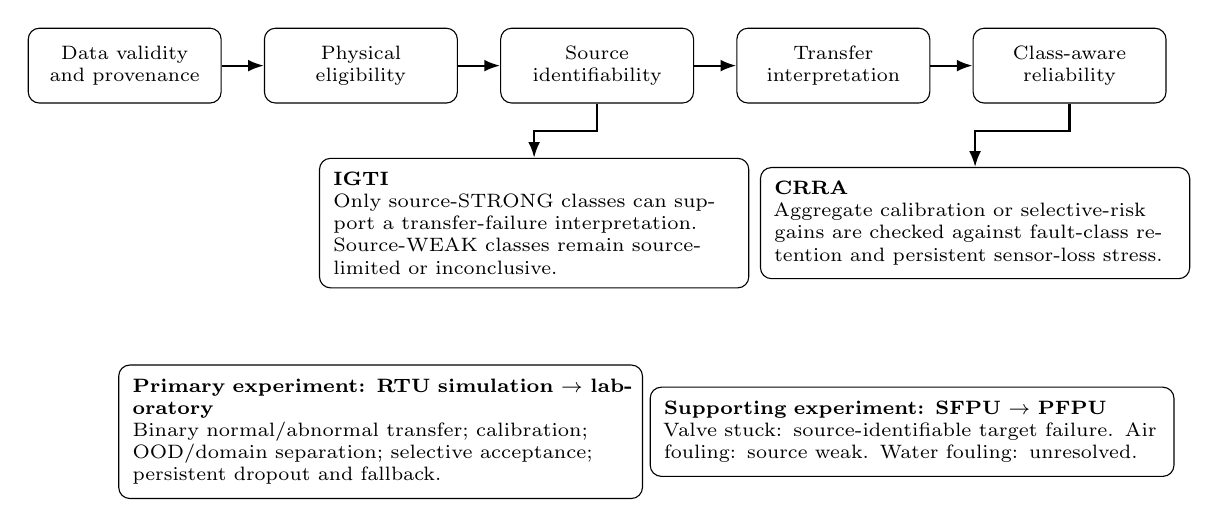
\begin{tikzpicture}[x=1cm,y=1cm,
  gate/.style={draw, rounded corners, align=center, minimum width=2.45cm, minimum height=0.95cm, font=\scriptsize},
  alg/.style={draw, rounded corners, align=left, text width=5.1cm, inner sep=5pt, font=\scriptsize},
  lane/.style={draw, rounded corners, align=left, text width=6.3cm, inner sep=5pt, font=\scriptsize},
  arr/.style={-{Latex[length=2mm]}, thick}
]
\node[gate] (g0) at (0,0) {Data validity\\and provenance};
\node[gate] (g1) at (3.0,0) {Physical\\eligibility};
\node[gate] (g2) at (6.0,0) {Source\\identifiability};
\node[gate] (g3) at (9.0,0) {Transfer\\interpretation};
\node[gate] (g4) at (12.0,0) {Class-aware\\reliability};
\draw[arr] (g0.east) -- (g1.west);
\draw[arr] (g1.east) -- (g2.west);
\draw[arr] (g2.east) -- (g3.west);
\draw[arr] (g3.east) -- (g4.west);

\node[alg] (igti) at (5.2,-2.0) {\textbf{IGTI}\\Only source-STRONG classes can support a transfer-failure interpretation. Source-WEAK classes remain source-limited or inconclusive.};
\node[alg] (crra) at (10.8,-2.0) {\textbf{CRRA}\\Aggregate calibration or selective-risk gains are checked against fault-class retention and persistent sensor-loss stress.};
\draw[arr] (g2.south) -- ++(0,-0.35) -| (igti.north);
\draw[arr] (g4.south) -- ++(0,-0.35) -| (crra.north);

\node[lane] (rtu) at (3.25,-4.65) {\textbf{Primary experiment: RTU simulation $\rightarrow$ laboratory}\\Binary normal/abnormal transfer; calibration; OOD/domain separation; selective acceptance; persistent dropout and fallback.};
\node[lane] (fp) at (10.0,-4.65) {\textbf{Supporting experiment: SFPU $\rightarrow$ PFPU}\\Valve stuck: source-identifiable target failure. Air fouling: source weak. Water fouling: unresolved.};
\end{tikzpicture}}
\caption{OIR-FDD evaluation and claim-governance framework. Data validity and physical eligibility precede source-identifiability auditing through IGTI. CRRA then evaluates whether aggregate confidence improvements remain credible after class retention and persistent sensor-loss stress are considered. The framework governs interpretation; it does not alter predictive models or perform target adaptation.}
\label{fig:oir}
\end{figure}

\subsection{Experimental settings and cohort contract}
The primary RTU experiment uses simulation as the source domain and laboratory operation as the target domain. Five frozen variables are shared: outdoor-air temperature, return-air temperature, supply-air temperature, supply-fan power, and total RTU power. The target fault mechanisms differ from the source fault mechanisms, so the task is binary normal-versus-abnormal transfer across data-generation domains, not closed-set same-fault transfer. Source-test support contains 471 normal and 14,370 abnormal windows; the laboratory target contains 221 normal and 611 abnormal windows.

The supporting cross-system experiment transfers four-class diagnosis from SFPU to PFPU. The retained classes are normal, air-side fouling, water-side fouling, and valve stuck. The PFPU target contains 8,756 normal, 461 air-fouling, 462 water-fouling, and 502 valve-stuck eligible windows. Room-temperature bias, valve leakage, and damper-stuck cases remain outside the frozen cohort because earlier integrity and observability audits did not support their use. Table~\ref{tab:contract} presents the reader-facing contract; detailed role-wise counts and sensor mappings are supplementary material.

\begin{table}[H]
\centering
\caption{Main experimental contract. Experiments are named by their physical source and target systems rather than internal development codes.}
\label{tab:contract}
\begin{threeparttable}
\small
\setlength{\tabcolsep}{4pt}
\begin{tabularx}{\textwidth}{>{\raggedright\arraybackslash}p{2.6cm}>{\raggedright\arraybackslash}X>{\raggedright\arraybackslash}p{4.0cm}}
\toprule
Experiment & Source-to-target diagnostic task & Evidence role \\
\midrule
RTU simulation $\rightarrow$ laboratory & Simulated RTU normal/fault episodes $\rightarrow$ laboratory RTU normal/abnormal operation. Binary normal vs. abnormal; source and target fault mechanisms differ. & Primary reliability test: transfer, calibration, OOD, abstention, and sensor loss. \\
SFPU $\rightarrow$ PFPU & Series fan-powered unit $\rightarrow$ parallel fan-powered unit. Four retained classes: normal, air-side fouling, water-side fouling, valve stuck. & Supporting source-identifiability and class-specific transfer analysis. \\
\bottomrule
\end{tabularx}
\begin{tablenotes}[flushleft]\footnotesize
\item Field RTU data are retained as protocol/deployment context only; no completed field efficacy result is claimed.
\end{tablenotes}
\end{threeparttable}
\end{table}

\subsection{Windowing, splits, and observability-aware eligibility}
Both experiments use a 300-min validity support composed of a 60-min context guard followed by a 240-min predictive interval, with a 60-min stride. Classical and MLP pipelines use channel means over the predictive interval; temporal models receive 24 ordered 10-min means. Splits are established before window generation, and no window crosses a role, purge, chronology segment, or frozen eligibility boundary.

The observability rules distinguish three objects: file-level fault presence, physical eligibility, and diagnostic eligibility. Known intervention information is used only for offline stratification and is never an input feature. Non-observable intervals remain in an all-monitored exposure ledger and are not relabeled as normal. Figure~\ref{fig:obs} shows the contract without using measured exposure durations.

\begin{figure}[H]
\centering
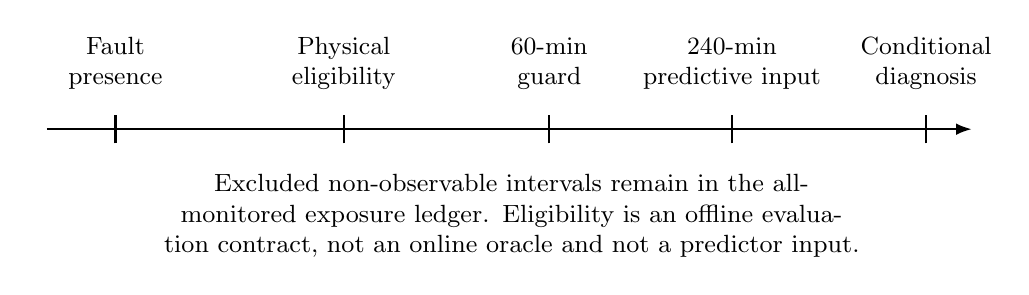
\begin{tikzpicture}[x=1.45cm,y=1cm, font=\small]
\draw[thick,-{Latex[length=2mm]}] (0,0) -- (8.1,0);
\foreach \x/\lab in {0.6/{Fault\\presence},2.6/{Physical\\eligibility},4.4/{60-min\\guard},6.0/{240-min\\predictive input},7.7/{Conditional\\diagnosis}} {
  \draw[thick] (\x,-0.18) -- (\x,0.18);
  \node[align=center, above=2mm] at (\x,0.18) {\lab};
}
\node[align=center, text width=12cm] at (4.05,-1.10) {Excluded non-observable intervals remain in the all-monitored exposure ledger. Eligibility is an offline evaluation contract, not an online oracle and not a predictor input.};
\end{tikzpicture}
\caption{Observability-aware window eligibility and evaluation contract. The 60-min guard protects chronology and role boundaries; the 240-min interval supplies the predictive input. The schematic is conceptual and does not encode empirical exposure duration.}
\label{fig:obs}
\end{figure}

\subsection{Baseline models and source-governed selection}
Eight baseline pipelines are retained: Logistic Regression (LR), Random Forest (RF), XGBoost, a multilayer perceptron (MLP), a one-dimensional convolutional neural network (1D-CNN), a temporal convolutional network (TCN), a long short-term memory network (LSTM), and Transformer. Later dropout analyses use four predeclared representative models (Random Forest, XGBoost, TCN, and Transformer). Source identifiability is audited with source-selected XGBoost, TCN, and Transformer configurations after a limited source-only balancing/capacity study. The comparisons therefore concern complete predictive pipelines rather than parameter-count-matched architecture effects. The manuscript uses each acronym only after its first full-name definition; internal experiment codes are confined to the supplementary and reproducibility materials.

\subsection{IGTI: Identifiability-Gated Transfer Interpretation}
Let $\mathcal{C}$ be the retained class set and $\mathcal{M}$ the source-selected model families. A class is labeled \textsc{Strong} when at least two selected families achieve source-test recall $\ge 0.70$ and precision $\ge 0.50$ under the frozen support guard. It is labeled \textsc{Weak} when at least two families have source recall $<0.50$; other cases remain unresolved. Algorithm~\ref{alg:igti} converts these source states and target outcomes into bounded transfer interpretations.

\begin{algorithm}[H]
\caption{Identifiability-Gated Transfer Interpretation (IGTI)}
\label{alg:igti}
\KwIn{Class set $\mathcal{C}$; eligible source/target supports; selected source models $\mathcal{M}$; source recall/precision; target recall; frozen support and STRONG/WEAK criteria.}
\KwOut{Class interpretation $z_c$ for every $c\in\mathcal{C}$.}
\ForEach{$c\in\mathcal{C}$}{
  verify source and target support under the frozen eligibility contract\;
  \If{support is insufficient}{
    $z_c\leftarrow$ \texttt{INCONCLUSIVE\_SUPPORT}\; \textbf{continue}\;
  }
  determine $\mathrm{source\_status}(c)$ from source-only recall and precision\;
  \eIf{$\mathrm{source\_status}(c)=\mathrm{STRONG}$ and target recognition is weak}{
    $z_c\leftarrow$ \texttt{SOURCE\_IDENTIFIABLE\_TARGET\_FAILURE}\;
  }{
    \eIf{$\mathrm{source\_status}(c)=\mathrm{WEAK}$ and target recognition is weak}{
      $z_c\leftarrow$ \texttt{SOURCE\_WEAK\_TARGET\_WEAK}\;
    }{
      $z_c\leftarrow$ \texttt{INCONCLUSIVE\_SUPPORT}\;
    }
  }
}
\Return{$\{z_c:c\in\mathcal{C}\}$}\;
\end{algorithm}

\subsection{CRRA: Class-Retention Reliability Audit}
CRRA combines established calibration and selective-prediction metrics with a class-retention gate and persistent-dropout stress. It does not introduce a new calibrator or uncertainty estimator. The audit uses balanced accuracy (BA), macro-F1, expected calibration error (ECE), Brier score, negative log-likelihood (NLL), and the area under the risk--coverage curve (AURC). Raw probabilities are evaluated alongside source-only parametric calibration: temperature scaling for multiclass/neural outputs and logistic/Platt calibration for binary classical outputs. Isotonic calibration is reported as not applicable when source support or score diversity fails the predeclared guard.

\begin{algorithm}[H]
\caption{Class-Retention Reliability Audit (CRRA)}
\label{alg:crra}
\KwIn{Raw and source-calibrated probabilities; source-derived acceptance rules; target labels for evaluation only; class set; persistent-dropout conditions; source-governed fallback variants.}
\KwOut{Calibration, selective, class-retention, and stress profiles plus a bounded reliability verdict.}
Evaluate BA, macro-F1, ECE, Brier score, NLL, risk-coverage, and AURC\;
\ForEach{declared threshold or descriptive coverage slice}{
  compute aggregate risk and coverage\;
  compute class coverage, accepted recall, and end-to-end recall\;
  \If{low aggregate risk coincides with zero accepted support for maintenance-relevant fault classes}{
    flag \texttt{SELECTIVE\_CLASS\_COLLAPSE}\;
  }
}
\ForEach{persistent sensor-dropout condition}{
  evaluate BA, macro-F1, ECE, and AURC\;
  evaluate mean-substitution fallback, source-dropout augmentation with a missingness indicator, and source-only channel-excluded fallback when defined\;
}
Aggregate worst-condition BA/F1 by minima and ECE/AURC by maxima using the frozen condition set\;
\If{an apparent aggregate improvement is contradicted by class collapse or adverse worst-condition stress}{
  do not promote the change to a reliability gain\;
}
\Return{complete class-aware reliability profile}\;
\end{algorithm}

\subsection{Reliability metrics and uncertainty scope}
Diagnosis is summarized by BA, macro-F1, and class recall. Calibration uses ECE, Brier score, and NLL. Selective prediction uses accepted risk, coverage, class coverage, accepted recall, end-to-end recall, and AURC. Persistent dropout removes a predeclared channel for an entire evaluation episode. Reported intervals describe algorithmic variability over five seeds on fixed cohorts; they are not confidence intervals over independent buildings, and overlapping windows are not treated as independent samples.

\section{Results}
\subsection{RTU simulation-to-laboratory transfer: diagnosis and confidence}
Source performance does not transfer uniformly. MLP source-test BA is 0.9256 but laboratory-target BA is 0.5000; Transformer changes from 0.8051 to 0.5196. Random Forest shows a smaller gap (0.4854 to 0.4737), but the weak source score prevents interpreting that small change as robustness. Target ECE is higher than source-test ECE for all eight frozen baseline pipelines. For example, Random Forest ECE rises from 0.0216 to 0.2055 and MLP ECE from 0.0534 to 0.2656. Figure~\ref{fig:rtu} and Table~\ref{tab:rtu} show the full comparison.

\begin{figure}[H]
\centering
\begin{subfigure}[t]{0.49\textwidth}
\centering
\includegraphics[width=\linewidth]{figures/F3a_BA.pdf}
\caption{Balanced accuracy.}
\end{subfigure}\hfill
\begin{subfigure}[t]{0.49\textwidth}
\centering
\includegraphics[width=\linewidth]{figures/F3b_ECE.pdf}
\caption{Expected calibration error.}
\end{subfigure}
\caption{RTU simulation-to-laboratory transfer for the eight frozen baseline pipelines. Stored intervals describe seed variability on fixed cohorts, not building-to-building uncertainty.}
\label{fig:rtu}
\end{figure}

\begin{table}[H]
\centering
\caption{RTU baseline transfer results. Higher BA is better; lower ECE is better.}
\label{tab:rtu}
\small
\begin{tabular}{lrrrr}
\toprule
Model & Source BA & Target BA & Source ECE & Target ECE\\
\midrule
Logistic Regression & 0.6265 & 0.5000 & 0.3574 & 0.7344\\
Random Forest        & 0.4854 & 0.4737 & 0.0216 & 0.2055\\
XGBoost              & 0.5506 & 0.4867 & 0.0197 & 0.2402\\
MLP                  & 0.9256 & 0.5000 & 0.0534 & 0.2656\\
1D-CNN               & 0.7347 & 0.5030 & 0.1951 & 0.2649\\
TCN                  & 0.7135 & 0.5052 & 0.1152 & 0.2660\\
LSTM                 & 0.7144 & 0.5001 & 0.1200 & 0.2657\\
Transformer          & 0.8051 & 0.5196 & 0.1000 & 0.2622\\
\bottomrule
\end{tabular}
\end{table}

The source-normal OOD companion rejects all target-normal and all target-fault windows, while target area under the receiver operating characteristic curve (AUROC) is only 0.5718. A separate domain classifier distinguishes simulation-normal from laboratory-normal windows with AUROC 1.0000. The combination is more consistent with strong generation-domain separation than with fault-specific novelty; high rejection of target faults therefore cannot be interpreted as successful unknown-fault detection.

\subsection{Calibration and selective prediction}
Source-only calibration has mixed effects rather than a uniform target benefit. Random Forest source-test ECE changes by -0.0020 after calibration but target ECE worsens by +0.0142. XGBoost shows the same sign reversal (-0.0007 at source test, +0.0029 on target). Transformer, by contrast, improves target ECE by -0.0849. Table~\ref{tab:cal} makes the heterogeneity explicit.

\begin{table}[H]
\centering
\caption{Source-only calibration: calibrated-minus-raw ECE. Negative values indicate improvement.}
\label{tab:cal}
\small
\begin{tabular}{lrr}
\toprule
Model & Source-test $\Delta$ECE & Target $\Delta$ECE\\
\midrule
Logistic Regression & -0.3107 & -0.0607\\
Random Forest        & -0.0020 &  0.0142\\
XGBoost              & -0.0007 &  0.0029\\
MLP                  & -0.0112 & -0.0016\\
1D-CNN               & -0.0231 & -0.0025\\
TCN                  & -0.0227 & -0.0103\\
LSTM                 & -0.0242 & -0.0113\\
Transformer          & -0.0580 & -0.0849\\
\bottomrule
\end{tabular}
\end{table}

The more consequential failure appears under abstention. In the SFPU-to-PFPU experiment, raw Random Forest reaches aggregate risk 0.0000 at a descriptive target-ranked 60\% coverage slice, yet air-side fouling, water-side fouling, and valve-stuck coverage are all 0.0000; only normal operation remains accepted. Figure~\ref{fig:selective} shows this counterexample together with the RTU calibration and threshold-transfer results. CRRA therefore labels the case selective class collapse rather than successful abstention.

\begin{figure}[H]
\centering
\begin{subfigure}[t]{0.52\textwidth}
\centering
\includegraphics[width=\linewidth]{figures/F4a_calibration.pdf}
\caption{Source-only calibration changes in ECE for the RTU baselines.}
\end{subfigure}\hfill
\begin{subfigure}[t]{0.45\textwidth}
\centering
\includegraphics[width=\linewidth]{figures/F4b_selective.pdf}
\caption{Class coverage at the descriptive 60\% target-ranked slice for the SFPU-to-PFPU Random Forest.}
\end{subfigure}
\caption{Calibration and selective-prediction evidence. Aggregate risk is zero in panel (b) while all retained fault classes are rejected.}
\label{fig:selective}
\end{figure}

\subsection{Persistent sensor loss and fallback}
Sensor loss changes different reliability metrics in different directions. For RTU XGBoost, total-power dropout lowers target BA by 0.0243 and increases AURC by 0.0972, while ECE improves by 0.0528. In the SFPU-to-PFPU example, Random Forest room-temperature dropout leaves BA and macro-F1 unchanged but increases ECE by 0.0741 and AURC by 0.0135. These cases show why robustness cannot be inferred from classification scores alone.

Source-governed fallback does not repair all dimensions. Mean-plus-indicator and channel-exclusion strategies improve some model/channel combinations while worsening calibration or AURC in others. Figure~\ref{fig:dropout} gives the complete RTU channel stress map, while Table~\ref{tab:worst} reports the predeclared worst-condition summaries.

\begin{figure}[H]
\centering
\includegraphics[width=0.95\textwidth]{figures/F6_sensor_dropout_labeled.pdf}
\caption{Persistent sensor-dropout stress in the RTU laboratory target. (a) Paired change in balanced accuracy (BA). (b) Paired change in expected calibration error (ECE). (c) Paired change in area under the risk--coverage curve (AURC). Columns correspond to the frozen RTU core sensors and rows to the predeclared representative model families; signed cell values show dropout minus clean performance.}
\label{fig:dropout}
\end{figure}

\begin{table}[H]
\centering
\caption{Worst-condition RTU reliability over the declared persistent-dropout condition set.}
\label{tab:worst}
\small
\begin{tabular}{lrrrr}
\toprule
Model & Worst BA & Worst F1 & Worst ECE & Worst AURC\\
\midrule
Random Forest & 0.4568 & 0.4229 & 0.2284 & 0.3885\\
XGBoost       & 0.4528 & 0.4161 & 0.2618 & 0.3983\\
TCN           & 0.4604 & 0.4234 & 0.2656 & 0.2709\\
Transformer   & 0.4142 & 0.3815 & 0.2661 & 0.3767\\
\bottomrule
\end{tabular}
\end{table}

\subsection{Source identifiability changes the meaning of target failure}
The supporting SFPU-to-PFPU experiment does not satisfy the frozen full four-class source-learnability criterion. The class-level diagnosis, however, is not uniform. Valve stuck is source identifiable: after source-only selection and balancing, source recall is approximately 0.89 across XGBoost, TCN, and Transformer, while target recall falls to 0.004--0.088. Air-side and water-side fouling behave differently. Air-versus-water pairwise discrimination on source test is near chance (LR AUROC 0.5000; XGBoost AUROC 0.5082), and the source class criteria remain weak or unresolved. IGTI therefore assigns three different scientific interpretations instead of calling every low target score a transfer failure.

\begin{figure}[H]
\centering
\begin{subfigure}[t]{0.49\textwidth}
\centering
\includegraphics[width=\linewidth]{figures/F5a_pairwise.pdf}
\caption{Source-only pairwise discrimination.}
\end{subfigure}\hfill
\begin{subfigure}[t]{0.49\textwidth}
\centering
\includegraphics[width=\linewidth]{figures/F5b_recall.pdf}
\caption{Source and target class recall for the selected model families.}
\end{subfigure}
\caption{Source identifiability and class-specific transfer interpretation for SFPU-to-PFPU diagnosis. Air-side versus water-side fouling remains near chance at source, whereas valve-stuck recognition is strong at source and collapses on target.}
\label{fig:ident}
\end{figure}

\begin{table}[H]
\centering
\caption{IGTI class-level interpretation for the retained fault mechanisms.}
\label{tab:igti}
\small
\begin{tabularx}{\textwidth}{lrrX}
\toprule
Fault & Mean source recall & Mean target recall & Interpretation\\
\midrule
Air-side fouling   & 0.5052 & 0.1137 & Source weak; target weak\\
Water-side fouling & 0.4932 & 0.0489 & Inconclusive support\\
Valve stuck        & 0.8913 & 0.0378 & Source-identifiable target failure\\
\bottomrule
\end{tabularx}
\end{table}

\subsection{Ablation and structural-control study}
The structural experiments were designed as an ablation family rather than a new graph-model competition. The evaluated representations are raw input, functional normalization, component-semantic alignment, physical graph, semantic graph, Brick-supported graph, and hybrid graph. Identity-edge and shuffled-edge hybrid controls test whether clean gains can be attributed to the intended topology. Internal development identifiers are retained only in the reproducibility package and supplementary records.

Table~\ref{tab:ablation} shows the central result. Some graph variants improve clean BA, macro-F1, or ECE, but those gains do not survive the reliability criteria. The hybrid graph reaches BA 0.2637 and ECE 0.0778, yet worst-channel ECE and AURC deteriorate to 0.5425 and 0.6393. The shuffled-edge hybrid control achieves much higher clean BA (0.4259) and macro-F1 (0.3472) than the documented hybrid graph while also improving ECE. This weakens a topology-specific explanation for the clean-score gains. The result is negative evidence for the tested structural priors, not a claim that graph-based HVAC FDD is generally ineffective.

\begin{table}[H]
\centering
\caption{Ablation and structural-control results for the SFPU-to-PFPU experiment. Lower ECE/AURC is better; higher BA/F1 is better.}
\label{tab:ablation}
\scriptsize
\resizebox{\textwidth}{!}{%
\begin{tabular}{lrrrrrr}
\toprule
Variant & BA & F1 & ECE & AURC & Worst-channel ECE & Worst-channel AURC\\
\midrule
Raw representation             & 0.2586 & 0.2380 & 0.0986 & 0.0161 & 0.1355 & 0.0332\\
Functional normalization      & 0.2500 & 0.2312 & 0.1371 & 0.0175 & 0.2113 & 0.2061\\
Component-semantic alignment        & 0.2500 & 0.2312 & 0.1373 & 0.0198 & 0.1854 & 0.2430\\
Physical graph        & 0.2673 & 0.2546 & 0.0753 & 0.0144 & 0.5508 & 0.6269\\
Semantic graph graph  & 0.2499 & 0.2311 & 0.1252 & 0.0140 & 0.1619 & 0.3496\\
Brick-supported graph & 0.2499 & 0.2312 & 0.1275 & 0.0139 & 0.3422 & 0.5142\\
Hybrid graph          & 0.2637 & 0.2532 & 0.0778 & 0.0144 & 0.5425 & 0.6393\\
Identity-edge hybrid control        & 0.2500 & 0.2312 & 0.1334 & 0.0128 & 0.2286 & 0.4024\\
Shuffled-edge hybrid control        & 0.4259 & 0.3472 & 0.0395 & 0.0111 & 0.1427 & 0.3135\\
\bottomrule
\end{tabular}}
\end{table}

\section{Discussion}
\subsection{Source identifiability is a prerequisite for a transfer-failure claim}
Cross-domain HVAC research has understandably focused on adaptation accuracy, source selection, and feature alignment \cite{lei2025,zhang2025source,ghalamsiah2025can,ghalamsiah2026graph}. The SFPU-to-PFPU results show why the source side deserves equal scrutiny. Valve-stuck recall is 0.890--0.892 on source test across XGBoost, TCN, and Transformer, but only 0.004--0.088 on PFPU. That contrast supports a genuine class-specific transfer-degradation interpretation. The fouling mechanisms behave differently: source-test air-versus-water discrimination is essentially chance (AUROC 0.500 for logistic regression and 0.508 for XGBoost), even though normal-versus-fouling AUROC is approximately 0.97. The supplementary source diagnostics (Table~S5 and Table~S6) therefore separate ``fault present'' from ``fault mechanism identifiable.

This distinction changes which intervention is scientifically justified. A domain-adaptation method evaluated on a class that is poorly separable at source may appear to ``fail under shift'' even when the limiting factor is the source representation or sensor contract. In the present source-capacity audit, class balancing raises mean source fault recall from roughly one third to about 0.63 for the selected families, yet the complete four-class task still misses the predeclared learnability criterion because the fouling mechanisms remain weak. Conversely, a strongly learned source distinction that disappears on target is precisely the case in which transfer adaptation becomes scientifically relevant. IGTI makes that separation explicit. It does not prove physical identifiability; it states what the frozen data and learner family support.

The result is consistent with long-standing diagnostic theory in which observability, isolability, and sensor reliability constrain what faults can be distinguished \cite{bhushan2000,yang2009}. What changes in OIR-FDD is the placement of that idea inside a modern cross-system data-driven evaluation: source identifiability is checked before a target degradation is promoted to a transfer-failure claim.

\subsection{Calibration and abstention must be interpreted with retained fault classes}
The RTU experiment reinforces the distinction between discrimination and confidence. Target ECE is higher than source-test ECE for all eight raw baseline pipelines, even though the size of the BA shift differs widely across models. For example, Random Forest changes from ECE 0.0216 to 0.2055, whereas MLP changes from 0.0534 to 0.2656. Source-only calibration is not uniformly corrective: Random Forest improves source-test ECE by 0.0020 but worsens target ECE by 0.0142, while Transformer target ECE improves by 0.0849. The complete calibration-support and selective diagnostics are reported in Supplementary Sections S2--S3. This mirrors broader evidence that calibration can deteriorate under dataset shift \cite{ovadia2019uncertainty,liang2023uq}. Source-only calibration partly repairs some models but worsens others, so no source calibration method can be treated as a target guarantee.

Selective prediction creates a different risk. At the descriptive 60\% target-ranked coverage slice, the SFPU-to-PFPU Random Forest reaches zero aggregate risk while accepting none of the retained fault classes; the accepted set is effectively normal operation. Figure~S1 shows how class coverage changes across 60--90\% ranked slices, making the collapse visible before any single risk value is interpreted. Standard risk-coverage analysis is therefore necessary but insufficient for an imbalanced maintenance task. The finding does not invalidate selective prediction \cite{geifman2017selective,geifman2019selectivenet}; it shows that the accepted population must be audited by class. CRRA operationalizes this by reporting class coverage, accepted recall, and end-to-end recall alongside aggregate risk.

The closest HVAC reliability comparator, Jiang \cite{jiang2026leakage}, also warns that confidence can be misleading under cross-domain deployment. The present contribution is complementary: rather than asking whether target support or adaptation should be trusted, CRRA asks whether the accepted predictions still contain the faults that the diagnostic service is meant to detect.

\subsection{Sensor availability is part of the diagnostic contract}
Sensor reviews emphasize that FDD performance depends on sensor placement, calibration, maintenance, and the information content of available measurements \cite{zhang2021sensor,hu2025sensorreview}. The present dropout results add a class-aware reliability perspective. Removing total RTU power from XGBoost changes target BA by $-0.0243$ and AURC by $+0.0972$ while ECE moves in the favorable direction by $-0.0528$. In the supporting experiment, room-temperature dropout leaves Random Forest BA and macro-F1 unchanged but worsens ECE by 0.0741 and AURC by 0.0135. These opposing movements are why the stress analysis reports discrimination, calibration, and selective ranking together rather than collapsing them into a single robustness score. A single headline metric would therefore tell an incomplete story.

This matters operationally because persistent channel loss differs from isolated missing cells. A failed BAS sensor removes an information source from every decision in the affected episode. Source-side missingness indicators or channel-excluded models can help, but the fallback experiments show that accuracy recovery and reliability recovery need not coincide. For the supporting TCN, the mean-plus-indicator fallback improves BA by 0.0868 relative to mean substitution while ECE and AURC recoveries are negative under the stored sign convention. Supplementary Section S4 reports the same comparison across the four predeclared representative model families in the RTU setting. This result complements online sensor-calibration work \cite{li2025voting}: fixing or virtualizing the sensor is one strategy; auditing diagnostic degradation when the measurement is absent is another.

\subsection{Structural priors require ablation evidence beyond clean accuracy}
Graph and ontology approaches provide valuable mechanisms for encoding equipment relations, causal structure, and building metadata \cite{balaji2016brick,zhang2022causal,ghalamsiah2026graph,li2026agentic}. The ablation results show, however, that clean-score improvement alone is not sufficient evidence that a structural prior improves reliability. The physical and hybrid graph variants improve some clean metrics but fail under worst-channel stress. Relative to the component-semantic graph reference, the hybrid graph improves clean BA by 0.0137 and macro-F1 by 0.0220 and lowers ECE by 0.0556, yet worst-class coverage decreases by 0.4855 and worst-channel ECE/AURC deteriorate by 0.3139/0.2370. The shuffled-edge hybrid control reaches clean BA 0.4259 and macro-F1 0.3472, both above the documented hybrid topology (0.2637/0.2532). Supplementary Section S6 retains the complete semantic and structural-control context.

The shuffled control is especially informative because it weakens a topology-specific causal story. It does not make shuffling a proposed solution; it shows that some apparent graph gains can arise without preserving the intended HVAC relations. This is why the graph results remain secondary in the manuscript. A future graph method should be required to improve not only target accuracy but also class retention, calibration, and sensor-loss robustness under matched training conditions.

\subsection{What OIR-FDD changes in benchmark reporting}
Table~\ref{tab:synthesis} summarizes the main evidence transitions. The framework does not replace established metrics or models. Its value is to prevent one metric from silently standing in for a stronger claim. A file-level fault label is not evidence that every window is diagnostically eligible. A low target score is not evidence of transfer failure without source identifiability. A low selective risk is not evidence of safe abstention when fault classes disappear. A clean graph gain is not evidence of structural reliability when shuffled topology or sensor loss reverses the conclusion.

\begin{table}[H]
\centering
\caption{Evidence-to-interpretation synthesis used in OIR-FDD.}
\label{tab:synthesis}
\small
\begin{tabularx}{\textwidth}{p{3.0cm}p{4.0cm}X}
\toprule
Observed evidence & What it supports & What it does not support automatically\\
\midrule
Fault file + eligible operating state & Conditional diagnosis cohort & Unique fault identifiability or deployment-wide efficacy\\
Strong source class + weak target class & Credible class-specific transfer degradation & Causal attribution to a single domain factor\\
Low aggregate selective risk & Low error among accepted predictions & Retention of fault classes or useful end-to-end diagnosis\\
Clean graph improvement & Better clean metric under the tested representation & Topology-specific benefit or robustness to missing sensors\\
Fallback accuracy recovery & Recovery of one discrimination metric & Recovery of calibration, ranking, or worst-condition reliability\\
\bottomrule
\end{tabularx}
\end{table}

For building-operation research, this claim-by-claim structure is consistent with the broader move from algorithm demonstrations toward field-relevant validation and interpretable deployment evidence \cite{shi2019review,andersen2024barriers,mosteiro2026dbn}. The current results remain bounded, but they show that evaluation design can change the scientific conclusion even when the underlying predictions are unchanged.

\section{Limitations}
The physical-system coverage is narrow. One simulation-to-laboratory RTU setting and one directional SFPU-to-PFPU setting do not constitute independent replication across a building population. Field RTU data remain protocol-level context, and no field false-alarm rate, detection delay, energy saving, comfort benefit, or maintenance-cost reduction is claimed.

The RTU experiment confounds several forms of novelty. Source and target differ in data-generation process, equipment realization, operating context, and fault mechanisms. The normal-domain classifier confirms strong domain separation but cannot identify which factor causes the transfer failure. Likewise, the SFPU-to-PFPU experiment contains limited independent fault episodes and operating-state confounding.

Observability masks are offline evaluation devices. They use known intervention information and frozen physical rules to define the conditional diagnosis cohort; they are not online oracles. Persistent-dropout evaluation retains the complete-data eligibility set, so the missing-sensor experiments assess predictive robustness on a fixed cohort rather than the online computability of the eligibility rule itself.

The source-capacity audit is limited, and final seed intervals are conditional on the selected configurations and fixed data. Temporal windows overlap, normal blocks can share a simulation run, and five training seeds are not independent buildings. The graph ablations also precede the later source-balancing audit, so they do not establish how a redesigned graph model would behave under the improved source-learning regime.

Finally, OIR-FDD, IGTI, and CRRA are evaluation methods, not predictive architectures. They do not provide formal safety guarantees, causal identification, or population-wide reliability bounds. Their role is to make the evidence boundary explicit for the experiments that were actually performed.

\section{Conclusion}
Cross-system HVAC fault diagnosis cannot be interpreted reliably from target accuracy alone. In the RTU simulation-to-laboratory experiment, diagnostic performance, calibration, OOD behavior, selective acceptance, and missing-sensor robustness degrade in different ways under the same target domain. In the SFPU-to-PFPU experiment, source identifiability changes the meaning of target failure: valve stuck is learned strongly at source and then largely lost on target, whereas the fouling mechanisms remain weak or unresolved before transfer.

OIR-FDD formalizes this layered evidence structure. IGTI prevents source-limited classes from being labeled as transfer failures, and CRRA prevents aggregate confidence improvements from being interpreted without checking class retention and sensor-loss stress. The structural ablation further shows that clean graph gains can fail to survive reliability controls and can even be exceeded by shuffled topology. The resulting message is deliberately bounded: physical eligibility, source discrimination, transfer performance, confidence, and sensing robustness require separate evidence. Future work can use the same framework to evaluate target adaptation, online observability, field deployment, or a dedicated reliability-aware predictive architecture on newly frozen external data.

\section*{CRediT authorship contribution statement}
\textbf{Chun-Jan Tseng:} Conceptualization, Funding acquisition, Methodology, Project administration, Supervision, Validation, Visualization, Writing - review \& editing.\\
\textbf{Yi-Kai Su:} Conceptualization, Data curation, Formal analysis, Investigation, Methodology, Software, Validation, Visualization, Writing - original draft.\\
\textbf{Ming-Han Chang:} Validation, Writing - review \& editing.

\section*{Data availability}
The study uses publicly released HVAC fault-detection datasets cited in the manuscript. The reproducibility package will be maintained at \url{https://github.com/ottolan0728/hvac-reliability-oir-fdd}. The repository is intended to contain analysis code, IGTI and CRRA audit utilities, split and eligibility manifests, figure-generation scripts, derived result tables, and non-restricted reproducibility artifacts. A versioned release can be archived through Zenodo after the repository is finalized.

\section*{Ethics}
This study analyzes publicly released HVAC operational datasets and does not recruit human participants. No personally identifiable information is used.

\section*{Acknowledgments}
The authors acknowledge the National Center for High-Performance Computing for providing computational resources and facilities used in this research.

\section*{Funding}
This research was supported by the National Science and Technology Council (NSTC), Taiwan, under Grant No. NSTC 115-2222-E-031-002. The funding source had no role in the study design; data collection, analysis, or interpretation; preparation of the manuscript; or the decision to submit the article for publication.

\section*{Declaration of competing interest}
The authors declare that they have no known competing financial interests or personal relationships that could have appeared to influence the work reported in this paper.

\section*{Declaration of generative AI and AI-assisted technologies in the manuscript preparation process}
During the preparation of this work, the authors used ChatGPT and Codex (OpenAI) for language refinement, literature checking, manuscript organization, and limited technical assistance. The authors reviewed and edited all AI-assisted content, verified the reported analyses and cited sources against the underlying evidence, and take full responsibility for the content of the article.

\bibliographystyle{elsarticle-num}
\bibliography{references}

\end{document}